\documentclass[10pt, letterpaper]{report}
% !TeX program = xelatex
%==================PREAMBOLO=======================%
\usepackage[utf8]{inputenc}
\usepackage{psvectorian}
\usepackage{pgfplots}
\usepackage[Rejne]{fncychap}
\usepackage[export]{adjustbox}
\usepackage[T1]{fontenc}
\usepackage{lmodern}
\usepackage[shortlabels]{enumitem}
\usepackage{moresize}
\usepackage{graphicx} % Required for inserting images
\usepackage{hyperref}
\usepackage{listings}
\usepackage[table,xcdraw]{xcolor}
\usepackage{amssymb}
\usepackage{amsmath}
\usepackage[italian]{babel}
\usepackage{nicefrac, xfrac}
\usepackage{tikz}
\usepackage{mathrsfs} 
\usepackage{titletoc}
\usepackage{fancyhdr}
\usepackage{psvectorian,lipsum}
\usepackage{fourier-orns}
\usepackage{lipsum}
\usepackage[paper=a4paper,left=25mm,right=25mm,bottom=25mm,top=25mm]{geometry}
\definecolor{light-gray}{gray}{0.95}
\definecolor{cop}{HTML}{f7ecd7}
\definecolor{copAut}{HTML}{ababab}
\definecolor{copAut2}{HTML}{c3c3e6}
\definecolor{purcop}{HTML}{d0d3db}
\definecolor{sapienza}{HTML}{660f1d}
\definecolor{lightSapienza}{HTML}{e3d3d5}
\definecolor{darkgreen}{HTML}{008000}
\definecolor{cartaRiciclata}{HTML}{fcfcf7}
\newcommand{\redText}[1]{\color{red}#1\color{black}}
\newcommand{\code}[1]{\colorbox{light-gray}{\texttt{#1}}}
\newcommand{\codee}[1]{\colorbox{white}{\texttt{#1}}}
\newcommand{\K}{{\mathbb K}}
\newcommand{\notimplies}{%
  \mathrel{{\ooalign{\hidewidth$\not\phantom{=}$\hidewidth\cr$\implies$}}}}
\newcommand{\flowerLine}{ \begin{center}\decofourleft\hphantom{ }\decoone\hphantom{ }\decofourright\hphantom{}\hphantom{aa}
\decofourleft\hphantom{ }\decoone\hphantom{ }\decofourright\hphantom{}\hphantom{aa}
\decofourleft\hphantom{ }\decoone\hphantom{ }\decofourright\hphantom{}\hphantom{aa}
\decofourleft\hphantom{ }\decoone\hphantom{ }\decofourright\hphantom{}\hphantom{aa} 
\decofourleft\hphantom{ }\decoone\hphantom{ }\decofourright\hphantom{}\hphantom{aa}
\decofourleft\hphantom{ }\decoone\hphantom{ }\decofourright\hphantom{}\hphantom{aa}
\decofourleft\hphantom{ }\decoone\hphantom{ }\decofourright\hphantom{}\hphantom{aa}
\decofourleft\hphantom{ }\decoone\hphantom{ }\decofourright\hphantom{}\hphantom{aa}
\decofourleft\hphantom{ }\decoone\hphantom{ }\decofourright\hphantom{}\hphantom{aa}
\end{center}}
\definecolor{g}{RGB}{60, 50, 50}
\newcommand{\textg}[1]{\color{g}{\textbf{#1}}\color{black}}
\newcommand{\teo}[1]{{\large\color{sapienza}\textbf{Teorema #1 :\hphantom{a}}}}
\newcommand{\defi}[1]{{\large\color{sapienza}\textbf{Definizione #1 :\hphantom{a}}}}
\newcommand{\claim}[1]{{\color{sapienza}\textbf{Claim #1 :\hphantom{a}}}}
\newcommand{\lemma}[1]{{\color{sapienza}\textbf{Lemma #1 :\hphantom{a}}}}
\newcommand{\dimo}[1]{{\color{sapienza}\textbf{Dimostrazione #1 :\hphantom{a}}}}
\newcommand{\prop}[1]{{\color{sapienza}\textbf{Proposizione #1 :\hphantom{a}}}}
\newcommand\greybox[1]{%
  \vskip\baselineskip%
  \par\noindent\colorbox{light-gray}{%
    \begin{minipage}{\textwidth}#1\end{minipage}%
  }%
  \vskip\baselineskip%
}
\newcommand\sapbox[1]{%
  \vskip\baselineskip%
  \par\noindent\colorbox{lightSapienza}{%
    \begin{minipage}{\textwidth}#1\end{minipage}%
  }%
  \vskip\baselineskip%
}

\newcommand{\Z}{{\mathbb Z}}
\newcommand{\blank}{{\sqcup}}
\newcommand{\R}{{\mathbb R}}
\newcommand{\N}{{\mathbb N}}
\newcommand{\C}{{\mathbb C}}
\newcommand{\Sn}{{\mathcal S_n}}
\newcommand{\An}{{\mathcal A_n}}
\newcommand{\E}{{\mathcal E}}
\newcommand{\B}{{\mathcal B}}
\newcommand{\mcm}{{\text{mcm}}}
\newcommand{\rg}{{\text{rg}}}
\newcommand{\ve}{{\bar v}}
\newcommand{\spaz}{{\text{\hphantom{aa}}}}
\newcommand{\MCD}{{\text{MCD}}}
\newcommand{\tc}{{\text{ tale che }}}
\newcommand{\supp}{{\text{Supp}}}
\newcommand{\acc}{\\\hphantom{}\\}
\newcommand{\aut}{{\text{Aut}}}
\newcommand{\Span}{{\text{Span}}}
\newcommand{\End}{{\text{End}}}
\newcommand{\cen}{{\text{Centro}}}
\newcommand{\norm}{{\unlhd}}
\newcommand{\ciclS}{{\left \langle }}
\newcommand{\ciclE}{{\right \rangle }}
\newcommand{\boxedMath}[1]{\begin{tabular}{|c|}\hline \texttt{#1} \\ \hline\end{tabular} :}
\newcommand{\shell}[1]{\colorbox{black}{\textcolor{white}{\texttt{#1}}}}
\newcommand{\eqImportante}[1]{\begin{center}\huge\lefthand\hphantom{a}
    \normalsize\texttt{#1}
    \hphantom{aaa}\huge\righthand\end{center}}

\fancyhf{}
\pagestyle{fancy}
\usepackage{pgf-pie}  
\usetikzlibrary{positioning}

\renewcommand{\headrule}{%
\vspace{-8pt}\hrulefill
\raisebox{-2.1pt}{\quad\decothreeleft\decotwo\decothreeright\quad}\hrulefill}

%sta roba serve per il codice C
\definecolor{mGreen}{rgb}{0,0.6,0}
\definecolor{mGray}{rgb}{0.5,0.5,0.5}
\definecolor{mPurple}{rgb}{0.58,0,0.82}
\definecolor{backgroundColour}{rgb}{0.95,0.95,0.92}

\lstdefinestyle{CStyle}{
    backgroundcolor=\color{backgroundColour},   
    commentstyle=\color{mGreen},
    keywordstyle=\color{magenta},
    numberstyle=\tiny\color{mGray},
    stringstyle=\color{mPurple},
    basicstyle=\footnotesize,
    breakatwhitespace=false,         
    breaklines=true,                 
    captionpos=b,                    
    keepspaces=true,                 
    numbers=left,                    
    numbersep=5pt,                  
    showspaces=false,                
    showstringspaces=false,
    showtabs=false,                  
    tabsize=2,
    language=C
}
\lstdefinestyle{CppStyle}{
    backgroundcolor=\color{backgroundColour},   
    commentstyle=\color{mGreen}\ttfamily,
    morecomment=[l][\color{magenta}]{\#}
    keywordstyle=\color{blue}\ttfamily,
    numberstyle=\tiny\color{mGray},
    stringstyle=\color{red}\ttfamily,
    basicstyle=\ttfamily,
    breakatwhitespace=false,         
    breaklines=true,                 
    captionpos=b,                    
    keepspaces=true,                 
    numbers=left,                    
    numbersep=5pt,                  
    showspaces=false,                
    showstringspaces=false,
    showtabs=false,                  
    tabsize=2,
    language=C
}
\lstset{language=C++,
                basicstyle=\ttfamily,
                keywordstyle=\color{blue}\ttfamily,
                stringstyle=\color{red}\ttfamily,
                commentstyle=\color{green}\ttfamily,
                morecomment=[l][\color{magenta}]{\#}
}
%fine roba che serve per il codice C
\usepackage{minted}
 %TOGLI COMMENTO SE USI XELATEX
%\usepackage{fontspec}
\title{Programmazione di Sistemi Multicore} %========TITOLO========%
\author{Marco Casu}
\date{\vspace{-5ex}}
\begin{document}

%==================COPERTINA=======================%
\begin{titlepage}
    \pagecolor{purcop}
\begin{center}
    %TOGLI COMMENTO SE USI XELATEX
   %\setmainfont{Palace Script MT}
   \Huge Marco Casu\acc
    %\setmainfont{Grand Casino}
     %TOGLI COMMENTO SE USI XELATEX
    %\setmainfont{h Halfroad}
    \HUGE \decothreeleft\hphantom{ }{\Huge\selectfont Programmazione di Sistemi Multicore}\hphantom{ }\decothreeright
     %TOGLI COMMENTO SE USI XELATEX
   % \setmainfont{Times New Roman}
\end{center}
\thispagestyle{empty}
\begin{figure}[h]
    \centering{
        %l'immagine deve avere una risoluzione 2048x2048
        
\includegraphics[width=1\textwidth ]{images/copertina.jpeg}
    }
\end{figure}
\vfill 
\centering 
\includegraphics[width=0.4\textwidth ]{../../preamble/Stemma_sapienza.png} \acc
\centering \Large \color{sapienza}Facoltà di Ingegneria dell'Informazione,
Informatica e Statistica\\
Dipartimento di Informatica
\end{titlepage}

%===================FINE COPERTINA======================%
\newpage
\pagecolor{cartaRiciclata}%\setmainfont{Algerian}
\large
Questo documento è distribuito sotto la licenza 
\color{blue}\href{https://www.gnu.org/licenses/fdl-1.3.txt}{GNU}\color{black},  
è un resoconto degli appunti (eventualmente integrati con libri di testo) tratti dalle lezioni del corso di Programmazione di Sistemi Multicore
\hphantom{a}per la laurea 
triennale in Informatica. Se dovessi notare errori, ti prego di segnalarmeli.
\vfill
\begin{figure}[h!]
    \raggedright
    
\includegraphics[width=0.4\textwidth,right ]{../../preamble/tomodachi.pdf} 
\end{figure}
\newpage %\setmainfont{Times New Roman}
\normalsize
\tableofcontents 
\newpage

%==================FOOTER e HEADER=======================%
\fancyhf{}
\fancyhead[L]{\nouppercase{\leftmark}}
\fancyhead[R]{Sezione \thesection}
\fancyfoot[C]{\thepage}
\fancyfoot[L]{Appunti di Prog. di Sistemi Multicore}
\fancyfoot[R]{ Marco Casu}
%\fancyfoot[R]{\setmainfont{Palace Script MT}\huge Marco Casu \setmainfont{Times New Roman}}
%==================FOOTER e HEADER=======================%

%Ricorda del comando \flowerLine per separare le sottosezioni. Le sezioni si separano nelle diverse pagine

%==================INIZIO======================%

\chapter{Parallelismo : Motivazioni}
\section{Introduzione}
In una \textit{GPU} (Graphics Processing Unit), nota anche come scheda video, ci sono circa 
80 miliardi di transistor, e vengono utilizzate per allenare i grossi modelli di intelligenza 
artificiale, i quali necessitano migliaia di GPU, non è un caso se \textit{Nvidia} ad oggi, con 
il boom dell'IA, è una delle aziende più quotate al mondo. Le GPU, e la loro 
programmazione, sono uno fra i principali argomenti di questo corso.\acc 
L'evoluzione dell'hardware, ha portato i grossi sistemi di computazione, ad essere formati da 
svariate unità di calcolo piuttosto che una singola unità molto potente, i processori stessi di uso comune, 
ad oggi sono composti da più \textit{core}.\acc 
La legge di Moore riguarda una stima empirica che mette in correlazione lo scorrere del tempo con 
l'aumentare della potenza di calcolo dei processori, se inizialmente, a partire dagli anni 70, tale potenza 
raddoppiava ogni due anni, ad oggi tale andamento è andato rallentando, raggiungendo un 
incremento 1.5 in 10 anni.
\begin{center}
    \includegraphics[width=300pt]{images/processor_trend.eps}
\end{center}
L'obbiettivo di costruire calcolatori sempre più potenti è dipeso dalla necessità dell'Uomo 
di risolvere problemi sempre più complessi, come ad esempio, la risoluzione del genoma umano.\acc 
Il motivo per il quale non è possibile costruire processori monolitici sempre più potenti, risiede 
in un \textit{limite fisico} riguardante la densità massima possibile dei transistor in 
un chip.\begin{enumerate}
    \item transistor più piccoli $\longrightarrow$ processori più veloci
    \item processori più veloci $\longrightarrow$ aumento del consumo energetico 
    \item aumento del consumo energetico $\longrightarrow$ aumento del calore 
    \item aumento del calore $\longrightarrow$ problemi di inaffidabilità dei transistor
\end{enumerate}
\flowerLine
\section{Modelli di Parallelismo}
L'informatico che intende scrivere del codice per un sistema multicore, deve esplicitamente 
sfruttare i diversi core, limitandosi a scrivere un codice sequenziale, non starebbe sfruttando a pieno 
l'hardware a disposizione, rendendo il processo meno efficiente di quanto potrebbe essere.\acc 
La maggior parte delle volte, un algoritmo sequenziale, non può essere direttamente tradotto in un 
algoritmo parallelo, per questo bisogna scrivere il codice facendo riferimento all'hardware di 
destinazione. Si consideri adesso il seguente codice sequenziale, che ha lo scopo di sommare 
$n$ numeri dati in input.
\begin{lstlisting}[style=CStyle]
    sum = 0;
    for(i=0; i<n; i++){
        x = compute_next_value(...);
        sum += x;
    }
\end{lstlisting}
Si vuole rendere tale algoritmo parallelo, sapendo di essere a disposizione di $p$ core.
\begin{lstlisting}[style=CStyle]
    local_sum = 0;
    first_index = ...;
    last_index = ...;
    for(local_i=first_index; first_index<last_index; local_i++){
        local_x = compute_next_value(...);
        local_sum += local_x;
    }
\end{lstlisting}
In tale esempio, ogni core possiede le sue variabili private non condivise con gli altri core, 
ed esegue indipendentemente il blocco di codice. Ogni core conterrà la somma
parziale di $\nicefrac{n}{p}$ valori.\acc 
\textbf{Esempio} (24 numeri, 8 core) :\begin{center}
    valori : $1,4,3,\;\;\;9,2,8,\;\;\;5,1,1,\;\;\;6,2,7,\;\;\;2,5,0,\;\;\;4,1,8,\;\;\;6,5,1,\;\;\;2,3,9$\acc 
    \begin{tabular}{|l|l|l|l|l|l|l|l|l|}
        \hline
        \rowcolor[HTML]{C0C0C0} 
        core & 0 & 1 & 2 & 3 & 4 & 5 & 6 & 7 \\ \hline
        \texttt{local\_sum}    & 8 & 19 & 7 & 15 & 7 & 13 & 12 & 14 \\ \hline
        \end{tabular}
\end{center}
A questo punto, per ottenere la somma totale, vi sarà un core \textit{master} che riceverà le somme 
parziali da tutti gli altri core, per poi eseguire la somma finale.
\begin{lstlisting}[style=CStyle]
    if(master){
        sum = local_sum;
        for c : core{
            if(c!=self){
                sum += c.local_sum;
            }
        }
    }else{
        send local_sum to master;
    }
\end{lstlisting}
Dividere i dati per poi far eseguire la stessa computazione ai diversi nodi è la forma più semplice 
di parallelismo. La soluzione adottata non è ideale, in quanto, in seguito al calcolo delle somme 
parziali, tutti i core escluso il master non staranno eseguendo calcoli. Una possibile 
idea alternativa è di far si che a coppie i nodi si condividano le somme parziali per poi calcolarne 
una somma comune, sviluppando uno scambio di dati ad albero, come mostrato in figura \ref{fig:tree_cores}.
\begin{figure}[h!]
    \centering
    \includegraphics[width=280pt]{images/tree.eps}
    \caption{calcolo somme a coppie}
    \label{fig:tree_cores}
\end{figure}\acc
Possiamo identificare due tipi di parallelismo :\begin{itemize}
    \item \textbf{parallelismo dei task} : fra i core vengono divise diverse attività che vengono 
    svolte autonomamente.
    \item \textbf{parallelismo dei dati} : i dati da elaborare vengono divisi, ogni core eseguirà 
    la stessa computazione ma su una porzione diversa dei dati.
\end{itemize}
Quando si scrive un programma parallelo bisogna prestare attenzione alla \textit{sincronizzazione} dei 
processi, in quanto potrebbero dover accedere ad una stessa area di memoria. Risulta cruciale 
saper mettere in \textit{comunicazione} i vari core, e suddividere equamente il 
\textit{carico di lavoro} fra di essi. Verranno considerate 4 diverse tecnologie per la programmazione 
multicore : \begin{itemize}
    \item \textit{MPI} (Message Passing Interface) [ libreria ]
    \item \textit{Posix} Threads [ libreria ]
    \item \textit{OpenMP} [ libreria e compilatore ]
    \item \textit{CUDA} [ libreria e compilatore ]
\end{itemize}
La programmazione delle GPU richiederà un diverso compilatore, e non il solito \texttt{gcc}, in quanto 
l'architettura della scheda video differisce da quella del processore, e con essa le istruzioni.\acc
I sistemi paralleli possono essere categorizzati sotto vari aspetti.\begin{itemize}
    \item \textbf{shared memory} : Tutti i core accedono ad un'area di memoria comune. L'accesso 
    e la sincronizzazione vanno gestiti con cautela.
    \item \textbf{distributed memory} : Ogni core ha un area di memoria privata, e la comunicazione 
    avviene attraverso un apposito canale per lo scambio dei messaggi. 
\end{itemize}
\begin{figure}[h!]
    \centering
    \includegraphics[width=280pt]{images/sdmem.eps}
    \caption{modelli di parallelismo}
    \label{fig:sdmem}
\end{figure}
Vi è un altra suddivisione nei sistemi paralleli :\begin{itemize}
    \item \textbf{MIMD} : Ogni core ha una control unit indipendente, diversi core possono eseguire 
    diverse istruzioni nello stesso momento.
    \item \textbf{SIMD} : Vi è un singolo program counter per tutti i core, che eseguono in maniera 
    parallela le stesse istruzioni. Due core non possono eseguire operazioni diverse nello stesso momento.
\end{itemize}
Le GPU hanno una struttura \textit{SIMD}.\begin{center}
    \begin{tabular}{c|
        >{\columncolor[HTML]{EFEFEF}}c |
        >{\columncolor[HTML]{EFEFEF}}c |}
        \cline{2-3}
                                                           & \cellcolor[HTML]{C0C0C0}shared memory & \cellcolor[HTML]{C0C0C0}distributed memory \\ \hline
        \multicolumn{1}{|c|}{\cellcolor[HTML]{C0C0C0}SIMD} & CUDA                                  &                                            \\ \hline
        \multicolumn{1}{|c|}{\cellcolor[HTML]{C0C0C0}MIMD} & Pthreads/OpenMP/CUDA                  & MPI                                        \\ \hline
        \end{tabular}
\end{center}
Fin'ora sono stati utilizzati 3 termini chiave riguardante i tipi di programmazione,
 sebbene non vi sia una definizione comunemente accettata, 
la seguente verrà adottata in tale contesto : \begin{itemize}
    \item \textit{concorrente} : più processi sono attivi in uno stesso momento 
    \item \textit{parallela} : diverse entità cooperative che operano in maniera ravvicinata per 
    un obbiettivo comune.
    \item \textit{distribuita} : diverse entità cooperative.
\end{itemize}
La programmazione parallela o distribuita implica che sia anche concorrente, non è vero il contrario.
\chapter{Memoria Distribuita : MPI}
\textit{MPI} è una libreria standard (avente varie implementazioni) necessaria allo sviluppo di codice multiprocesso 
a memoria distribuita. Precisamente, ogni core ha una memoria privata inaccessibile dall'esterno, e la comunicazione 
avviene attraverso una rete di interconnesione, (ad esempio, un bus), tale modello è detto \textbf{message 
passing}.
\section{La libreria OpenMpi}
Alla compilazione ed avvio di un programma che sfrutta MPI, ogni core eseguirà il programma, sarà la logica 
di esso a suddividere il carico di lavoro, tramite i costrutti decisionali. Verrà utilizzata un'implementazione 
nota come \textit{openMpi}, è possibile installare la libreria su sistemi operativi linux tramite il comando \acc
    \shell{sudo apt-get install libopenmpi-dev}
\acc
Il seguente esempio, mostra un programma che scrive sulla console una stringa, e tramite MPI, tale processo è avviato 
su ogni core.
\begin{lstlisting}[style=CStyle]
    #include <stdio.h>
    #include <mpi.h>
    //voglio lanciare il programma su piu unita di calcolo
    int main(int argc, char **argv){
        int p = MPI_Init(NULL,NULL); 
        //Il parametro in output di MPI_Init e' uno status sull'errore
        if(p == MPI_SUCCESS){
        
        }else{
            printf("qualcosa e' andato storto");
            MPI_Abort(MPI_COMM_WORLD,p);
            //Con MPI_Abort tutti i processi su tutti i core avviati verranno terminati 
        }
        printf("hello world");
        MPI_Finalize(); //Serve per terminare la libreria
        return 0;
    }
\end{lstlisting}
I programmi MPI non vengono compilati con \shell{gcc}, ma con \shell{mpicc}\acc 
\shell{mpicc hello\_world.c -o hello\_world.out}
\acc
Una volta ottenuto l'eseguibile, è possibile lanciare il programma con \shell{mpirun} specificando 
il numero di core sulla quale verrà eseguito il programma, tale numero, se non specificato con apposite flag, 
deve essere minore o uguale al numero di core fisici presenti sulla macchina.\acc 
\shell{mpirun -n 4 hello\_world.out}
\acc 
Ogni funzione della libreria ha una dicitura che inizia con \textit{"MPI\_"}. Ogni funzione di libreria deve essere chiamata 
fra \begin{itemize}
    \item \code{MPI\_Init} - configurazione ed avviamento della libreria 
    \item \code{MPI\_Finalize} - chiusura e deallocazione della memoria 
\end{itemize}
Tali righe stabiliscono il blocco di codice in cui verranno eseguite funzioni MPI.
\flowerLine 
\section{Rank e Comunicazione}
Ogni processo MPI è univocamente identificato da un numero intero detto \textit{rank}, se $p$ processi sono 
attivi, avranno gli identificatori $1,2\dots,p-1$.\acc  Un \textbf{comunicatore} è un insieme di processi, i quali hanno 
la possibilità di scambiarsi messaggi, si può pensare ad un comunicatore come un etichetta, e processi con la stessa 
etichetta possono comunicare fra loro. 
È identificabile nel codice tramite la struttura dati \code{MPI\_Comm}, e all'avvio di MPI, viene sempre 
definito un comunicatore di default \code{MPI\_COMM\_WORLD} che contiene tutti i processi.\acc 
L'identificatore di ogni processo è in realtà relativo ad ogni comunicatore, due processi diversi possono condividere il 
rank se relativo a comunicatori diversi. Ci sono due funzioni importanti che riguardano questi ultimi\begin{itemize}
    \item \code{int MPI\_Comm\_rank(MPI\_Comm comm, int *rank)} : Prende in input un comunicatore ed un numero intero, e 
    salva dentro tale numero il rank del processo chiamante relativo al comunicatore dato.
    \item \code{int MPI\_Comm\_size(MPI\_Comm comm, int *size)} : Prende in input un comunicatore ed un numero intero, e 
    salva dentro tale intero il numero di processi all'interno del comunicatore.
\end{itemize}
\begin{lstlisting}[style=CStyle]
    #include <stdio.h>
    #include <mpi.h>
    //voglio lanciare il programma su piu unita di calcolo
    int main(int argc, char **argv){
        int p = MPI_Init(NULL,NULL); 
        //Il parametro in output di MPI_Init e' uno status sull'errore
        if(p == MPI_SUCCESS){
        
        }else{
            printf("qualcosa e' andato storto");
            MPI_Abort(MPI_COMM_WORLD,p);
            //Con MPI_Abort tutti i processi su tutti i core avviati verranno terminati 
        }
        int size;
        MPI_Comm_size(MPI_COMM_WORLD, &size);
        int rank;
        MPI_Comm_rank(MPI_COMM_WORLD, &rank);
        printf("hello world, im the process %d/%d",rank,size);
        MPI_Finalize(); //Serve per terminare la libreria
        return 0;
    }
\end{lstlisting}
La comunicazione avviene tramite due funzioni, il cui comportamento è simile alla comunicazione tramite \code{pipe}.\acc 
L'inzio dei messagi avviene tramite \code{int MPI\_Send}, i cui parametri sono\begin{itemize}
    \item \code{void* msg\_buf\_p} l'area di memoria da trasferire al processo destinatario 
    \item \code{int msg\_size} il numero di elementi (non l'occupazione in byte) del messaggio da trasferire 
    \item \code{MPI\_Datatype msg\_type} il tipo di elemento da trasferire. Sono definiti dei tipi standard che 
    incorporano tutti i tipi più comuni del \textit{C}
    \item \code{int dest} il rank del processo destinatario
    \item \code{int tag} un tag da dare al messaggio per identificarlo 
    \item \code{MPI\_Comm communicator} il comunicatore  su cui avviene la comunicazione
\end{itemize}
Può dipendere dall'implementazione, ma solitamente quando un processo fa una \code{MPI\_Send}, si arresta finché 
il messaggio inviato non viene ricevuto dal destinatario, allo stesso modo, un destinatario che si appresta a ricevere 
un messaggio viene arrestato fino al ricevimento. Le chiamate di comunicazione MPI sono quindi bloccanti. \acc 
Per ricevere dati, viene utilizzata la chiamata \code{MPI\_Recv}  i cui parametri sono\begin{itemize}
    \item \code{void* msg\_buf\_p} l'area di memoria su cui verrà salvato il messaggio 
    \item \code{int buf\_size} il numero di elementi (non l'occupazione in byte) del messaggio da ricevere 
    \item  \code{MPI\_Datatype buf\_type} il tipo di elemento da ricevere
    \item \code{int source} il rank del processo mittente
    \item \code{int tag} il tag del messaggio da ricevere
    \item \code{MPI\_Comm communicator} il comunicatore su cui avviene la comunicazione
    \item \code{MPI\_Status* status} lo status riguardante l'esito della comunicazione
\end{itemize}
OpenMpi definisce la seguente lista di tipi \code{MPI\_Datatype} :\begin{center}
    \begin{tabular}{|c|c|}
        \hline
        \rowcolor[HTML]{EFEFEF} 
        \texttt{MPI\_CHAR }           & carattere                  \\ \hline
        \texttt{MPI\_INT }            & intero                     \\ \hline
        \rowcolor[HTML]{EFEFEF} 
        \texttt{MPI\_FLOAT  }         & float a singola precisione \\ \hline
        \texttt{MPI\_DOUBLE  }        & float a doppia precisione  \\ \hline
        \rowcolor[HTML]{EFEFEF} 
        \texttt{MPI\_LONG }           & intero long                \\ \hline
        \texttt{MPI\_SHORT }          & intero short               \\ \hline
        \rowcolor[HTML]{EFEFEF} 
        \texttt{MPI\_UNSIGNED\_CHAR}  & carattere senza segno      \\ \hline
        \texttt{MPI\_UNSIGNED\_INT }  & intero senza segno         \\ \hline
        \rowcolor[HTML]{EFEFEF} 
        \texttt{MPI\_UNSIGNED\_LONG}  & intero long senza segno    \\ \hline
        \texttt{MPI\_UNSIGNED\_SHORT} & intero short senza segno   \\ \hline
        \end{tabular}
\end{center}
Il seguente programma fa si che ogni processo invii un messaggio al processo di rank 0, e quest'ultimo lo stampi 
a schermo.
\begin{lstlisting}[style=CStyle]
#include <stdio.h>
#include <mpi.h>

int main(int argc, char **argv)
{
    int p = MPI_Init(NULL, NULL);
    // Il parametro in output di MPI_Init e' uno status sull'errore
    if (p != MPI_SUCCESS)
    {
        printf("qualcosa e' andato storto");
        MPI_Abort(MPI_COMM_WORLD, p);
        // Con MPI_Abort tutti i processi su tutti i core avviati verranno terminati
    }
    int size;
    MPI_Comm_size(MPI_COMM_WORLD, &size);
    int str_size = 256;
    int rank;

    MPI_Comm_rank(MPI_COMM_WORLD, &rank);
    if (rank == 0)
    {
        printf("hello world, i am process 0. I will recive and print.\n", rank, size);
        char str[str_size];
        for (int i = 1; i < size; i++)
        {
            MPI_Recv(str, str_size, MPI_CHAR, i, 0, MPI_COMM_WORLD, MPI_STATUS_IGNORE);
            printf("(STRING RECIVED) : %s", str);
        }
    }
    else
    {
        char str[str_size];
        sprintf(str, "hello world, i am process %d of %d\n", rank, size);
        // Si invia al processo 0
        MPI_Send(str, str_size, MPI_CHAR, 0, 0, MPI_COMM_WORLD);
    }

    MPI_Finalize(); // Serve per terminare la libreria
    return 0;
}
\end{lstlisting}
Quando un processo esegue una \code{MPI\_Recv}, fra i vari messaggi, viene cercato quello di cui matchano il tag, il 
comunicatore, ed il mittente, lo scopo del \code{tag} è quello di essere un ulteriore separatore logico per 
la comunicazione. Anche i tipi dei messaggi devono combaciare, inoltre il numero di byte da ricevere deve essere 
maggiore o uguale al numero di byte inviati 
$$ ByteRecv\ge ByteSent$$
Nella chiamata \code{MPI\_Recv}, i campi \code{source} e \code{tag} possono essere riempiti con, rispettivamente,
\code{MPI\_ANY\_SOURCE} e \code{MPI\_ANY\_TAG} per non eseguire il controllo su mittente e tag nel ricevimento. 
È comunque possibile sapere qual'è il mittente, dato che tale informazione è salvata nel campo \code{MPI\_Status}.
\flowerLine 
\section{Design di Programmi Paralleli}
Data la specifica di un programma, quali sono le regole da seguire per partizionare il carico di lavoro fra i vari 
processi? Non esistono delle regole adatte ad ogni evenienza, ma è è stata definita una metodologia largamente generica, 
la \textbf{Foster's methodology}.
\begin{figure}[h!]
    \centering
    \includegraphics[width=0.9\textwidth]{images/foster.eps}
    \caption{Foster's methodology}
    \label{fig:foster}
\end{figure}
\begin{enumerate}
    \item \textit{Partizionamento} : si identificano delle attività di base indipendenti fra loro che possono essere
    eseguite in parallelo.
    \item \textit{Comunicazione} : determinare quali sono le attività stabilite nel punto precedente che per essere 
    eseguite necessitano di uno scambio di messaggi. 
    \item \textit{Aggregazione} : identificare le attività precedentemente stabilite che devono necessariamente essere 
    eseguite in sequenza, ed aggregarle in un unica attività.
    \item \textit{Mapping} : assegnare ai vari processi le attività definite in precedenza in modo che il carico di 
    lavoro sia uniformemente distribuito. Idealmente la comunicazione deve essere ridotta al minimo.
\end{enumerate}
\subsection{Pattern di Design Parallelo}
La struttura di un programma parallelo può essere definita secondo due pattern, si può dire che esistono due modi 
di \textit{parallelizzare} un programma \begin{itemize}
    \item \textbf{GPLS (Globally Parallel, Locally Sequential)} : L'applicazione vede diversi task sequenziali venire eseguiti in parallelo. 
    \item \textbf{GSLP (Globally Sequential, Locally Parallel)} : L'applicazione segue uno specifico "flusso" di esecuzione sequenziale, di cui 
    alcune parti vengono eseguite in parallelo.
\end{itemize}
\begin{figure}[h!]
    \centering
    \includegraphics[width=0.6\textwidth]{images/GPLSoGSLP.eps}
    \caption{GPLS e GSLP}
    \label{fig:GPLSoGSLP}
\end{figure}
\subsubsection{Esempi di GPLS}\begin{itemize}
    \item \textbf{Single Program Multiple Data} : La logica dell'applicazione viene mantenuta in un unico 
    eseguibile, tipicamente il programma segue la seguente struttura\begin{enumerate}
        \item Inizializzazione del programma 
        \item Ottenimento degli identificatori 
        \item Esecuzione del programma in diverse ramificazioni in base ai core coinvolti 
        \item Terminazione del programma
    \end{enumerate}
    \item \textbf{Multiple Program Multiple Data} : Quando la memoria da utilizzare è elevata è necessario suddividere 
    il carico su più programmi, che spesso vengono eseguiti su differenti piattaforme.
    \item \textbf{Master-Worker} : Ogni processo può essere \begin{itemize}
    \item Worker - Esegue la computazione
        \item Master - Gestisce il carico di lavoro e lo assegna ai processi worker, colleziona i risultati ottenuti 
        da questi ultimi e si occupa spesso delle operazioni di I/O o interazione con l'utente.
    \end{itemize}
    \item \textbf{Map-Reduce} : Una versione modificata del paradigma Master-Worker, in cui i nodi 
    worker eseguono due tipi di operazioni \begin{itemize}
        \item Map : Esegue la computazione su un insieme di dati che risulta in un insieme di risultati parziali (ad esempio, 
        esegue la somma su ogni elemento di un vettore) 
        \item Reduce : Colleziona i risultati parziali e ne deriva un risultato finale (ad esempio, somma tutti gli elementi di un 
        vettore ottenendo un unico scalare)
    \end{itemize}
\end{itemize}
\subsubsection{Esempi di GSLP}\begin{itemize}
    \item \textbf{Fork-Join} : C'è un unico "padre" in cui avviene l'esecuzione, quando necessario, 
    tale padre potrebbe eseguire una \code{fork} generando dei nodi figli, che eseguono la computazione 
    per poi terminare, facendo si che il padre continui.
    \item \textbf{Loop-Parallelism} : Risulta estremamente semplice da utilizzare e viene spesso applicata 
    quando un programma sequenziale deve essere adattato al multiprocesso. Consiste nel parallelizzare ogni 
    esecuzione di un ciclo \code{for}, è necessario che le iterazione però siano indipendenti fra loro.
\end{itemize}
\begin{lstlisting}[style=CStyle]
    //Esempio di Fork-Join
    mergesort(A,lo,hi){
        if lo < hi{
            mid = lo + (hi-lo) / 2 
            fork mergesort(A,lo,mid)
            mergesort(A,mid,hi)

            join 
            merge(A,lo,mid,hi)
        }
    }
\end{lstlisting}
\end{document}
